\documentclass[11pt,a4paper]{article}
\usepackage[T1]{fontenc}
\usepackage[utf8]{inputenc}
\usepackage{lmodern}
\usepackage[a4paper,margin=25mm]{geometry}
\usepackage{amsmath,amssymb,bm}
\usepackage{graphicx,booktabs,array}
\usepackage{needspace,float}
\usepackage{listings,xcolor}
\usepackage[hidelinks]{hyperref}
\usepackage{fancyhdr}
\pagestyle{fancy}
\fancyhf{}
\fancyhead[L]{\small Numerical Methods for the Heat Equation}
\fancyfoot[C]{\thepage}
\setlength{\headheight}{14pt}
\setlength{\parindent}{0pt}
\setlength{\parskip}{6pt}
\setlength{\emergencystretch}{2em}
\makeatletter
\let\tableinput\@@input
\makeatother
\newcommand{\task}[2]{\Needspace{6\baselineskip}\section*{Task #1: #2}\addcontentsline{toc}{section}{Task #1: #2}}
\newcommand{\partsol}[1]{\Needspace{4\baselineskip}\subsection*{(#1)}}
\newcommand{\dd}{\mathrm{d}}
\newcommand{\ii}{\mathrm{i}}
\newcommand{\lap}{\nabla^2}
\newcommand{\norminf}[1]{\left\|#1\right\|_\infty}
\newcommand{\normh}[1]{\left\|#1\right\|_{2,h}}
\lstset{basicstyle=\ttfamily\footnotesize,breaklines=true,columns=fullflexible,
  keepspaces=true,frame=single,rulecolor=\color{black!25},showstringspaces=false,
  tabsize=4}
\graphicspath{{figures/}}
\begin{document}
\begin{center}
{\LARGE\bfseries Numerical Methods for the Heat Equation}\par
\vspace{5pt}
{\large Detailed solutions to the background-notes tasks}
\end{center}
\vspace{4pt}
This document follows the task numbering in \emph{Numerical Methods for the Heat Equation}.
All 26 tasks are answered, including the optional Task 6.5. Numerical tables and plots are
computed results; the supporting programs and raw data are supplied with the LaTeX source.

\textbf{Notation.} The temperature is $u$, thermal diffusivity is $\alpha>0$, and grid nodes are
$x_i=i\Delta x$, $y_j=j\Delta y$, $t_n=n\Delta t$.
The superscript in $u^n_{i,j}$ denotes a time level, not a power.
For a square uniform grid, $\Delta x=\Delta y=h$ and
$r=\alpha\Delta t/h^2$. All Taylor expansions below assume the function has the bounded
derivatives required by the stated remainder.

\task{1.1}{Checking the mean-value formula}
We must prove that the average temperature on a small circle satisfies
\[
\frac{1}{2\pi}\int_0^{2\pi}u(x+\rho\cos\varphi,y+\rho\sin\varphi)\,\dd\varphi
=u(x,y)+\frac{\rho^2}{4}\lap u(x,y)+O(\rho^4).
\]
Here the circle radius is denoted by $\rho$, to distinguish it from the time-step parameter $r$ used later.

\textbf{Step 1: expand near the centre.}
Set $a=\rho\cos\varphi$, $b=\rho\sin\varphi$. With derivatives evaluated at $(x,y)$,
\begin{align*}
u(x+a,y+b)={}&u+a u_x+b u_y
+\frac12\bigl(a^2u_{xx}+2ab u_{xy}+b^2u_{yy}\bigr)\\
&+\frac16\bigl(a^3u_{xxx}+3a^2b u_{xxy}+3ab^2u_{xyy}+b^3u_{yyy}\bigr)
+O(\rho^4).
\end{align*}
The problem asks us to compute the second-order terms. The cubic terms are displayed as well
to justify the stated $O(\rho^4)$ remainder: a second-order expansion alone would give only
an $O(\rho^3)$ pointwise remainder.

\textbf{Step 2: average the constant and linear terms.}
The average of $u$ is $u$. Also,
\[
\int_0^{2\pi}\cos\varphi\,\dd\varphi
=\int_0^{2\pi}\sin\varphi\,\dd\varphi=0,
\]
so the linear terms contribute nothing.

\textbf{Step 3: average the quadratic terms.}
Using
\[
\int_0^{2\pi}\cos^2\varphi\,\dd\varphi
=\int_0^{2\pi}\sin^2\varphi\,\dd\varphi=\pi,
\qquad \int_0^{2\pi}\cos\varphi\sin\varphi\,\dd\varphi=0,
\]
the quadratic contribution is
\[
\frac{1}{2\pi}\frac{\rho^2}{2}
\bigl(\pi u_{xx}+0+\pi u_{yy}\bigr)
=\frac{\rho^2}{4}(u_{xx}+u_{yy}).
\]

\textbf{Step 4: account for the remainder.}
Each cubic monomial changes sign under $\varphi\mapsto\varphi+\pi$, so its integral
over a full circle is zero. The remaining term is uniformly $O(\rho^4)$ when $u$ has bounded
fourth derivatives near the circle. Its average is also $O(\rho^4)$. Therefore
\[
\boxed{\ \text{circle average}=u+\frac{\rho^2}{4}\lap u+O(\rho^4).\ }
\]
Thus a positive Laplacian means that the nearby surroundings are warmer on average than the
centre. In the heat equation, this makes the centre warm up.

\task{1.2}{Dimensional analysis}
\partsol{a}
Write $[L]$ for length units and $[\mathrm{time}]$ for time units. Thermal diffusivity has units
$[\alpha]=[L]^2/[\mathrm{time}]$. Consequently,
\[
\left[\frac{\alpha t}{L^2}\right]
=\frac{([L]^2/[\mathrm{time}])[\mathrm{time}]}{[L]^2}=1.
\]
Therefore $\alpha t/L^2$ is dimensionless.

\partsol{b}
Seek a time scale of the form $\alpha^a L^b$. Its units are
\[
[\alpha^aL^b]=[L]^{2a+b}[\mathrm{time}]^{-a}.
\]
Matching the units of time requires $-a=1$ and $2a+b=0$.
Hence $a=-1$, $b=2$, and the only such monomial, up to a dimensionless constant, is
\[
\boxed{\tau=\frac{L^2}{\alpha}.}
\]
If $L$ and $\alpha$ are the only dimensional parameters, a spreading time must have the form
$t_{\mathrm{spread}}=C L^2/\alpha$. The dimensionless constant $C$ depends on the shape,
boundary conditions, and what is meant by ``spread''; dimensional analysis does not determine it.

For $L=10\,\mathrm{cm}=0.10\,\mathrm{m}$, using the diffusivities supplied in the notes,
\begin{align*}
\tau_{\mathrm{copper}}&=\frac{0.10^2}{1.1\times10^{-4}}
\simeq90.9\,\mathrm{s}\simeq1.52\,\mathrm{min},\\
\tau_{\mathrm{steel}}&=\frac{0.10^2}{1.3\times10^{-5}}
\simeq769.2\,\mathrm{s}\simeq12.8\,\mathrm{min}.
\end{align*}
Steel's characteristic time is approximately $8.46$ times larger. This agrees with the
expectation that heat spreads faster through copper. These are diffusion scales, not exact
times at which the plate reaches equilibrium.

\partsol{c}
Define
\[
\hat x=x/L,\qquad \hat y=y/L,\qquad \hat t=\alpha t/L^2,
\]
and let $\hat u(\hat x,\hat y,\hat t)=u(L\hat x,L\hat y,L^2\hat t/\alpha)$.
By the chain rule,
\[
u_t=\frac{\alpha}{L^2}\hat u_{\hat t},\qquad
u_{xx}=\frac{1}{L^2}\hat u_{\hat x\hat x},\qquad
u_{yy}=\frac{1}{L^2}\hat u_{\hat y\hat y}.
\]
Substitution in $u_t=\alpha(u_{xx}+u_{yy})$ and cancellation of $\alpha/L^2$ give
\[
\boxed{\hat u_{\hat t}=\hat u_{\hat x\hat x}+\hat u_{\hat y\hat y}.}
\]
Neither $\alpha$ nor $L$ appears in this equation. A solver for unit diffusivity on a unit square
therefore describes any geometrically similar square plate after rescaling coordinates and time:
$x=L\hat x$, $y=L\hat y$, $t=(L^2/\alpha)\hat t$. Initial and boundary data must be transformed
too. A rectangle with unequal sides retains its aspect ratio; scaling does not change its shape.

\task{1.3}{Fourier modes}
Let
\[
\beta_x=\frac{m\pi}{L_x},\qquad \beta_y=\frac{n\pi}{L_y},\qquad
\lambda=\alpha(\beta_x^2+\beta_y^2),
\]
where $m,n$ are positive integers. The proposed function is
\[
u_{mn}(x,y,t)=\sin(\beta_xx)\sin(\beta_yy)e^{-\lambda t}.
\]
\textbf{Step 1: differentiate in time.}
The sine factors are independent of time, so
\[
(u_{mn})_t=-\lambda u_{mn}.
\]
\textbf{Step 2: differentiate twice in each spatial direction.}
Since $(\sin(\beta x))''=-\beta^2\sin(\beta x)$,
\[
(u_{mn})_{xx}=-\beta_x^2u_{mn},\qquad
(u_{mn})_{yy}=-\beta_y^2u_{mn}.
\]
It follows that
\[
\alpha\lap u_{mn}
=-\alpha(\beta_x^2+\beta_y^2)u_{mn}
=-\lambda u_{mn}=(u_{mn})_t.
\]
\textbf{Step 3: check every boundary.}
At $x=0$, the first sine is zero; at $x=L_x$, it is $\sin(m\pi)=0$.
Similarly the second sine vanishes at $y=0,L_y$. Thus all four Dirichlet conditions hold.

\textbf{Step 4: evaluate the initial data.}
At $t=0$ the exponential is one, so
\[
\boxed{u_0(x,y)=\sin\!\left(\frac{m\pi x}{L_x}\right)
\sin\!\left(\frac{n\pi y}{L_y}\right).}
\]
Each mode retains its spatial shape while its amplitude decays exponentially. The decay rate
increases quadratically with mode number, explaining why fine spatial oscillations disappear
more rapidly than broad temperature variations.

\task{2.1}{Taylor expansions}
All derivatives in this task are evaluated at $x$.
\partsol{a}
Taylor's formula gives
\[
\boxed{f(x+h)=f+hf'+\frac{h^2}{2}f''+\frac{h^3}{6}f'''
+\frac{h^4}{24}f^{(4)}+O(h^5).}
\]
\partsol{b}
Replace $h$ by $-h$:
\[
\boxed{f(x-h)=f-hf'+\frac{h^2}{2}f''-\frac{h^3}{6}f'''
+\frac{h^4}{24}f^{(4)}+O(h^5).}
\]
Terms containing odd powers of $h$ change sign, since $(-h)^k=-h^k$ for odd $k$.
Even powers do not change sign. This distinction makes it possible to cancel selected Taylor
terms by adding or subtracting symmetric samples.
\partsol{c}
Replace $h$ by $2h$:
\begin{align*}
f(x+2h)&=f+2hf'+\frac{(2h)^2}{2}f''+\frac{(2h)^3}{6}f'''
+\frac{(2h)^4}{24}f^{(4)}+O((2h)^5)\\
&=\boxed{f+2hf'+2h^2f''+\frac43h^3f'''+\frac23h^4f^{(4)}+O(h^5).}
\end{align*}
The factor $2^5$ in the remainder is constant, so it is absorbed in the $O(h^5)$ notation.

\task{3.1}{The backward difference}
The backward approximation is
\[
D_-f(x)=\frac{f(x)-f(x-h)}{h}.
\]
Insert the expansion from Task 2.1(b):
\begin{align*}
f(x)-f(x-h)
&=hf'-\frac{h^2}{2}f''+\frac{h^3}{6}f'''-\frac{h^4}{24}f^{(4)}+O(h^5),\\
D_-f(x)&=f'-\frac{h}{2}f''+\frac{h^2}{6}f'''-\frac{h^3}{24}f^{(4)}+O(h^4).
\end{align*}
Thus, defining truncation error as approximation minus exact derivative,
\[
\boxed{D_-f(x)-f'(x)=-\frac{h}{2}f''(x)+O(h^2)=O(h).}
\]
The method is first-order accurate. For a generic function the leading error is proportional to
$h$, so halving $h$ approximately halves the error. Its leading sign is opposite to that of
the forward difference. A particular function or point can have $f''(x)=0$ and a smaller error;
this does not change the general order of the formula.

\task{3.2}{A finite difference for the second derivative}
\partsol{a}
Add the symmetric Taylor expansions instead of subtracting them:
\[
f(x+h)+f(x-h)=2f(x)+h^2f''(x)+\frac{h^4}{12}f^{(4)}(x)+O(h^6).
\]
Here the stronger $O(h^6)$ form follows by expanding through degree five and cancelling odd
terms, assuming sufficient smoothness. Subtract $2f(x)$ and divide by $h^2$:
\[
\boxed{D_2f(x)=\frac{f(x-h)-2f(x)+f(x+h)}{h^2}\approx f''(x).}
\]
The same coefficients follow systematically from
\[
D_2f=\frac{af(x-h)+bf(x)+cf(x+h)}{h^2}.
\]
After expansion, cancelling the constant and first derivative and matching $f''$ gives
\[
a+b+c=0,\qquad -a+c=0,\qquad \frac{a+c}{2}=1.
\]
Hence $a=c=1$ and $b=-2$.

\partsol{b}
The expansion above gives
\[
\boxed{D_2f(x)-f''(x)=\frac{h^2}{12}f^{(4)}(x)+O(h^4).}
\]
The leading truncation error is $h^2 f^{(4)}(x)/12$, so the method is second-order accurate.
If only the expansions through degree four with $O(h^5)$ remainders are used, one obtains
the same leading term and an $O(h^3)$ remainder, already sufficient to establish order two.

\partsol{c}
For $f(x)=\sin x$,
\[
f''(1)=-\sin1\simeq-0.8414709848078965,\qquad f^{(4)}(1)=\sin1.
\]
The experiment evaluates the three-point quotient directly in double precision.
\begin{center}
\begin{tabular}{rrrr}
\toprule
$h$ & $D_2f(1)$ & $|D_2f(1)-f''(1)|$ & Previous error / error\\
\midrule
\tableinput{tables/task_3_2.tex}
\bottomrule
\end{tabular}
\end{center}
The ratios approach $4=2^2$, confirming second-order accuracy. The error is positive before
taking the absolute value, as predicted by $h^2\sin1/12$: the approximation is slightly less
negative than the exact second derivative.

\task{3.3}{Sanity checks on the second derivative}
\partsol{a}
For a constant function $f(x)=1$,
\[
D_2f(x)=\frac{1-2+1}{h^2}=0.
\]
For $f(x)=x$,
\[
D_2f(x)=\frac{(x-h)-2x+(x+h)}{h^2}=0.
\]
For $f(x)=x^2$,
\begin{align*}
D_2f(x)&=\frac{(x-h)^2-2x^2+(x+h)^2}{h^2}\\
&=\frac{(x^2-2xh+h^2)-2x^2+(x^2+2xh+h^2)}{h^2}=2.
\end{align*}
These are the exact derivatives: constants and straight lines have no curvature, and $x^2$
has curvature $2$. For a consistent fixed-coefficient three-point formula divided by $h^2$,
the corresponding Taylor moment conditions must cancel constants and linear terms and normalize
the quadratic term. A failure of these tests reveals an incorrect coefficient or scaling.

\partsol{b}
The coefficient sum is
\[
\frac{1-2+1}{h^2}=0.
\]
Consequently adding the same constant temperature to all three samples leaves the computed
second derivative unchanged. This expresses the fact that curvature depends on relative values,
not on the choice of temperature origin.

\partsol{c}
Define the neighbour average by
\[
\bar f=\frac{f(x-h)+f(x+h)}{2}.
\]
Then
\[
\boxed{D_2f(x)=\frac{2}{h^2}\bigl(\bar f-f(x)\bigr).}
\]
The second difference is positive if the centre is below its neighbours' average, negative if
it is above that average, and zero if they balance. In heat diffusion, this determines whether
the centre warms or cools.

\task{3.4}{The discrete Laplacian}
\partsol{a}
Hold $y=y_j$ fixed and apply the second difference in $x$:
\[
\boxed{u_{xx}(x_i,y_j)\approx
\frac{u_{i+1,j}-2u_{i,j}+u_{i-1,j}}{\Delta x^2}.}
\]
\partsol{b}
Hold $x=x_i$ fixed and apply it in $y$:
\[
\boxed{u_{yy}(x_i,y_j)\approx
\frac{u_{i,j+1}-2u_{i,j}+u_{i,j-1}}{\Delta y^2}.}
\]
\partsol{c}
Adding gives the discrete Laplacian
\[
\boxed{\lap_hu_{i,j}=
\frac{u_{i+1,j}-2u_{i,j}+u_{i-1,j}}{\Delta x^2}
+\frac{u_{i,j+1}-2u_{i,j}+u_{i,j-1}}{\Delta y^2}.}
\]
For samples of a smooth exact function, its error is
\[
\lap_hu-\lap u
=\frac{\Delta x^2}{12}u_{xxxx}+\frac{\Delta y^2}{12}u_{yyyy}
+O(\Delta x^4+\Delta y^4).
\]
Thus the spatial approximation is $O(\Delta x^2+\Delta y^2)$.
No mixed derivative is needed because the Laplacian itself is the sum of the two pure second derivatives.

\partsol{d}
If $\Delta x=\Delta y=h$,
\[
\boxed{\lap_hu_{i,j}=
\frac{u_{i-1,j}+u_{i+1,j}+u_{i,j-1}+u_{i,j+1}-4u_{i,j}}{h^2}.}
\]
\partsol{e}
The following array marks the five nodes and their weights. Empty positions are unused;
the common factor is $1/h^2$.
\[
\frac{1}{h^2}
\begin{array}{c|ccc}
 & i-1&i&i+1\\\hline
j+1&&1&\\
j&1&-4&1\\
j-1&&1&
\end{array}
\qquad
\begin{array}{c}
\text{north: }(i,j+1)\\
\text{west, centre, east: }(i-1,j),(i,j),(i+1,j)\\
\text{south: }(i,j-1)
\end{array}
\]
For unequal spacings the west/east weights are $1/\Delta x^2$, the north/south weights
are $1/\Delta y^2$, and the centre weight is $-2/\Delta x^2-2/\Delta y^2$.
Diagonal nodes such as $(i+1,j+1)$ do not belong to this stencil.

\partsol{f}
Let $\bar u_4$ be the arithmetic mean of the four neighbouring samples. Then
\[
\lap_hu_{i,j}=\frac{4}{h^2}(\bar u_4-u_{i,j}),
\qquad
\bar u_4=u_{i,j}+\frac{h^2}{4}\lap u+O(h^4).
\]
Task 1.1 gives the same leading expression for the circular average at radius $h$.
Both measure the difference between the centre and its surroundings. The averages need not
coincide exactly: the four-point average samples only the coordinate directions, and their
fourth-order terms can differ.

\task{3.5}{Where round-off takes over}
We repeat the direct quotient in Task 3.2 at $x=1$ for $h=10^{-1},\ldots,10^{-10}$.
The computed values are:
\begin{center}
\begin{tabular}{rrr}
\toprule
$h$ & Computed $D_2\sin(1)$ & Absolute error\\
\midrule
\tableinput{tables/task_3_5.tex}
\bottomrule
\end{tabular}
\end{center}
\begin{figure}[H]
\centering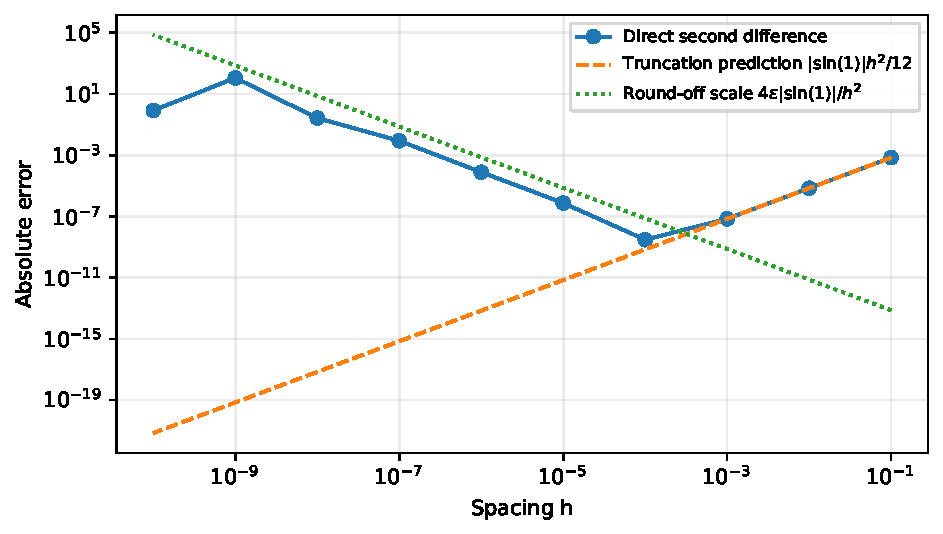
\includegraphics[width=.88\linewidth]{task_3_5_roundoff.pdf}
\caption{Direct second-difference error in double precision. The round-off curve is a scale
estimate, not a pointwise bound; cancellation makes the measured error irregular.}
\end{figure}
\textbf{Observed transition.} In this run the smallest error among the sampled spacings occurs
at $h=10^{-4}$. Reducing $h$ to $10^{-5}$ increases the error sharply. Thus the transition
is near $10^{-4}$, with the precise location depending on floating-point rounding.

\textbf{Why this happens.} The truncation error is approximately
$C h^2$, where $C=|\sin1|/12$. Each sampled function value contains rounding error.
The coefficients $1,-2,1$ combine errors of scale $\epsilon |f|$, and division by $h^2$
amplifies them. A useful model is
\[
E(h)\approx C h^2+\frac{D\epsilon}{h^2},\qquad \epsilon\simeq2.22\times10^{-16},
\]
where $D$ is a function-dependent constant of order one. Differentiating this model gives
\[
2Ch-2D\epsilon h^{-3}=0
\quad\Longrightarrow\quad
h_{\mathrm{opt}}^4=\frac{D\epsilon}{C}.
\]
Therefore $h_{\mathrm{opt}}$ has scale $\epsilon^{1/4}$, roughly $10^{-4}$.
The $\sqrt\epsilon$ scale discussed for the forward \emph{first} derivative does not apply here:
the second derivative has both a different truncation error and a division by $h^2$.

For extremely small $h$, nearly equal sine values are subtracted, and the numerator may round
to zero or to a small multiple of machine precision. Dividing that unreliable residual by $h^2$
can produce a very large error. Smaller spacing is therefore useful only until round-off
overtakes truncation error. The exact last digits of this table can vary between math libraries.

\task{4.1}{Experiments with forward and backward Euler}
We solve
\[
u'=-50u,\qquad u(0)=1,\qquad 0\le t\le1.
\]
The exact solution is $u(t)=e^{-50t}$; in particular,
$u(1)=e^{-50}\simeq1.928749847963918\times10^{-22}$.

\partsol{a}
Forward Euler replaces the derivative by a forward difference:
\[
\frac{u^{n+1}-u^n}{\Delta t}=-50u^n
\quad\Longrightarrow\quad
\boxed{u^{n+1}=(1-50\Delta t)u^n.}
\]
To reach $t=1$ exactly, choose an integer $M$ and use $\Delta t=1/M$.
The following implementation is the recurrence used in the experiment:
\begin{lstlisting}[language=Python]
def forward_euler(M):
    dt = 1.0 / M
    u = 1.0
    for n in range(M):
        u = (1.0 - 50.0 * dt) * u
    return u
\end{lstlisting}
Since each step multiplies by the same factor $g=1-50\Delta t$, an independent formula is
$u^n=g^n$. This provides a direct check on the program.

\partsol{b}
Boundedness for arbitrarily many steps requires $|g|\le1$:
\[
-1\le1-50\Delta t\le1
\quad\Longrightarrow\quad
\boxed{0\le\Delta t\le0.04.}
\]
The numerical experiment compares steps on both sides of this limit. The final backward-Euler
column is discussed in part (d).
\begin{center}
\small
\begin{tabular}{rrrrr}
\toprule
$M$ & $\Delta t$ & $g_{\mathrm{FE}}$ & $u^M_{\mathrm{FE}}$ & $u^M_{\mathrm{BE}}$\\
\midrule
\tableinput{tables/task_4_1_stability.tex}
\bottomrule
\end{tabular}
\end{center}
For $\Delta t=0.05$, the factor is $-1.5$ and the magnitude grows. For
$\Delta t=1/24>0.04$, growth is slower but still present because $|g|>1$.
At the endpoint $\Delta t=0.04$, $g=-1$: the iterates alternate between $+1$ and $-1$.
They are bounded, so this endpoint is stable in the boundedness sense, but it does not reproduce
the physical decay. Strict decay requires $0<\Delta t<0.04$.
For $\Delta t=1/26$, the signs alternate while the magnitude decreases.
For $\Delta t=0.02$, $g=0$, so the numerical solution becomes zero after the first step.
That last fact is a property of this recurrence, not exact integration of the ODE.

\begin{figure}[H]
\centering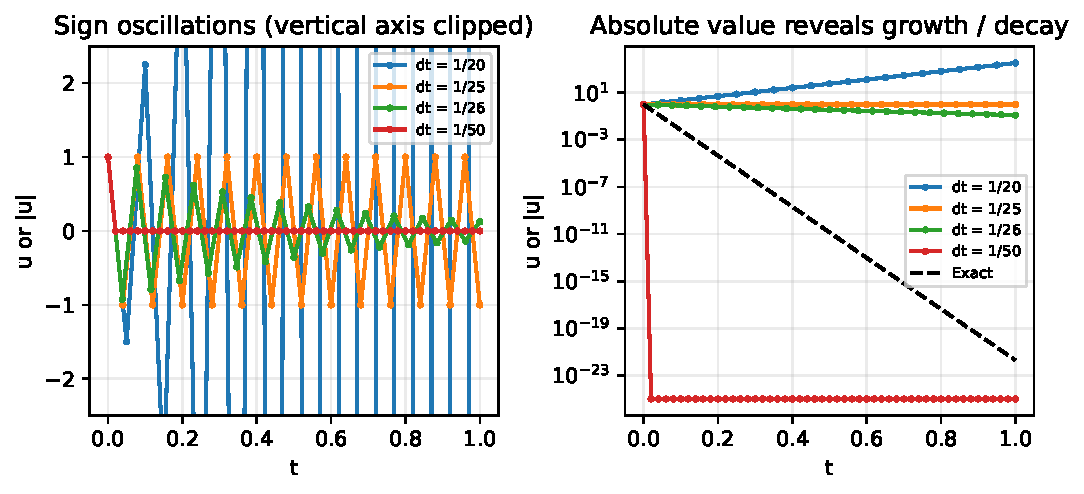
\includegraphics[width=\linewidth]{task_4_1_stability.pdf}
\caption{Forward Euler near its stability threshold. The left panel shows sign changes;
the logarithmic right panel shows whether their magnitudes grow or decay.}
\end{figure}
A finite observation interval alone cannot prove stability: a factor slightly larger than one
may not produce a spectacular blow-up by $t=1$. The recurrence and the bound on $|g|$ establish
the threshold exactly.

\partsol{c}
At the common final time $T=1$, define
\[
E(\Delta t)=\left|u^M-e^{-50}\right|,\qquad
p_{\mathrm{obs}}=\log_2\frac{E(\Delta t)}{E(\Delta t/2)}.
\]
We use sufficiently small steps to enter the asymptotic regime:
\begin{center}
\small
\begin{tabular}{rrrrr}
\toprule
$M$ & $\Delta t$ & $u^M$ & Absolute error & $p_{\mathrm{obs}}$\\
\midrule
\tableinput{tables/task_4_1.tex}
\bottomrule
\end{tabular}
\end{center}
The observed orders approach one. The very small absolute errors reflect the fact that the
exact final temperature is already about $10^{-22}$. They should be interpreted relative to
that final value, rather than as an indication that coarse steps are exceptionally accurate.

To explain why the fine steps in the table are useful, expand the logarithm for $50\Delta t<1$:
\begin{align*}
\log(1-50\Delta t)&=-50\Delta t-\frac{50^2}{2}\Delta t^2+O(\Delta t^3),\\
\log u^M&=\frac{1}{\Delta t}\log(1-50\Delta t)
=-50-1250\Delta t+O(\Delta t^2).
\end{align*}
Thus
\[
u^M=e^{-50}\bigl(1-1250\Delta t+O(\Delta t^2)\bigr),
\qquad
\boxed{E(\Delta t)=1250e^{-50}\Delta t+O(\Delta t^2).}
\]
The leading error is proportional to $\Delta t$. To see its asymptotic ratio clearly,
$1250\Delta t$ should be small, which is a stronger requirement than stability alone.
\begin{figure}[H]
\centering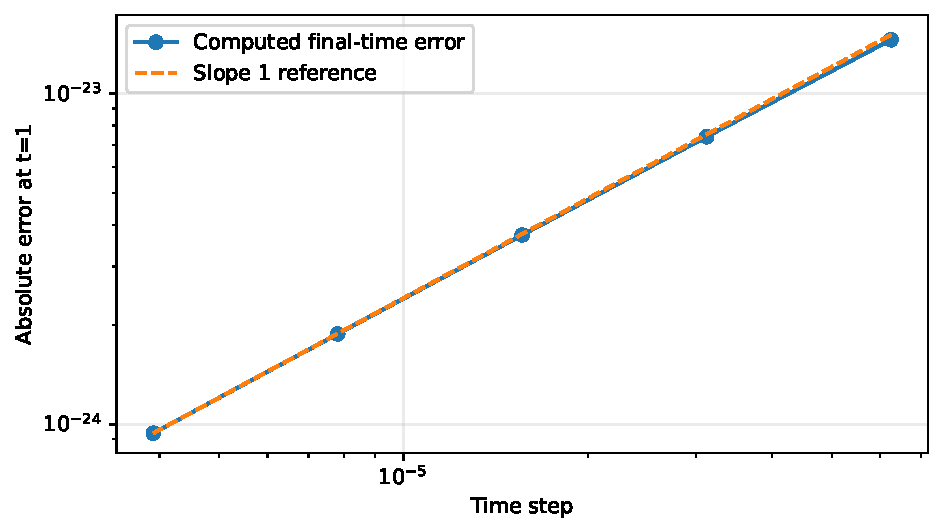
\includegraphics[width=.85\linewidth]{task_4_1_order.pdf}
\caption{Final-time forward-Euler error. The computed curve approaches the slope-one reference.}
\end{figure}

\partsol{d}
Backward Euler evaluates the right-hand side at the new time:
\[
\frac{u^{n+1}-u^n}{\Delta t}=-50u^{n+1}.
\]
Rearranging,
\[
(1+50\Delta t)u^{n+1}=u^n,
\qquad
\boxed{u^{n+1}=\frac{u^n}{1+50\Delta t}.}
\]
An implementation changes only the multiplication factor:
\begin{lstlisting}[language=Python]
def backward_euler(M):
    dt = 1.0 / M
    u = 1.0
    for n in range(M):
        u = u / (1.0 + 50.0 * dt)
    return u
\end{lstlisting}
For every $\Delta t>0$, $0<g_{\mathrm{BE}}=1/(1+50\Delta t)<1$.
Therefore the sequence stays positive and decreases, whatever the step size: there is
\emph{no finite upper stability limit}. The table includes steps larger than the forward-Euler
limit; they remain bounded with backward Euler.

Unconditional stability does not imply arbitrary accuracy. For example, taking one step with
$\Delta t=1$ gives $u^1=1/51\simeq0.01961$, far larger than $e^{-50}$.
Backward Euler is also first-order accurate; indeed,
\[
\log u^M=-\frac{1}{\Delta t}\log(1+50\Delta t)
=-50+1250\Delta t+O(\Delta t^2).
\]
It approaches the exact final value from above as the step is refined.

\task{5.1}{Warm-up: the one-dimensional heat equation}
Consider $u_t=\alpha u_{xx}$ for $0<x<L$ with prescribed boundary temperatures.
Let $x_i=i\Delta x$, where $\Delta x=L/N$.

\partsol{a}
Replace the spatial derivative while retaining continuous time. For $1\le i\le N-1$,
\[
\boxed{\frac{\dd u_i}{\dd t}
=\alpha\frac{u_{i+1}(t)-2u_i(t)+u_{i-1}(t)}{\Delta x^2}.}
\]
This is a system of $N-1$ ODEs. The boundary values $u_0(t)$ and $u_N(t)$ are known data;
they enter the equations adjacent to the boundaries.

\partsol{b}
Apply forward Euler to each ODE:
\[
\frac{u_i^{n+1}-u_i^n}{\Delta t}
=\alpha\frac{u_{i+1}^n-2u_i^n+u_{i-1}^n}{\Delta x^2}.
\]
Solving for the new value yields
\[
\boxed{u_i^{n+1}=u_i^n+
\frac{\alpha\Delta t}{\Delta x^2}
\bigl(u_{i+1}^n-2u_i^n+u_{i-1}^n\bigr).}
\]
Only level-$n$ values occur on the right, so every new interior value can be computed
independently once the old level is available.

\partsol{c}
The dimensionless combination is
\[
\boxed{r_x=\frac{\alpha\Delta t}{\Delta x^2}.}
\]
Its units cancel exactly as in Task 1.2(a), with $t$ replaced by $\Delta t$ and $L$ by
$\Delta x$. It compares the time step with the diffusion time $\Delta x^2/\alpha$
across a single grid cell. The update becomes
\[
u_i^{n+1}=(1-2r_x)u_i^n+r_xu_{i-1}^n+r_xu_{i+1}^n.
\]
Task 6.2 will show that this explicit scheme requires $r_x\le1/2$.

\task{5.2}{The two-dimensional update rule}
\partsol{a}
At an interior node the semi-discrete ODE is
\[
\frac{\dd u_{i,j}}{\dd t}
=\alpha\left[
\frac{u_{i+1,j}-2u_{i,j}+u_{i-1,j}}{\Delta x^2}
+\frac{u_{i,j+1}-2u_{i,j}+u_{i,j-1}}{\Delta y^2}\right].
\]
Define $r_x=\alpha\Delta t/\Delta x^2$ and $r_y=\alpha\Delta t/\Delta y^2$.
Applying forward Euler gives
\begin{align*}
\boxed{\begin{aligned}
u_{i,j}^{n+1}=u_{i,j}^n
&+r_x\bigl(u_{i+1,j}^n-2u_{i,j}^n+u_{i-1,j}^n\bigr)\\
&+r_y\bigl(u_{i,j+1}^n-2u_{i,j}^n+u_{i,j-1}^n\bigr).
\end{aligned}}
\end{align*}
The scheme is used at $1\le i\le N_x-1$, $1\le j\le N_y-1$.
Dirichlet boundary nodes are set to the prescribed data rather than updated by this formula.

\partsol{b}
For equal spacings $h$, let $r=\alpha\Delta t/h^2$. Then
\[
\boxed{u_{i,j}^{n+1}=u_{i,j}^n+r\left(
u_{i-1,j}^n+u_{i+1,j}^n+u_{i,j-1}^n+u_{i,j+1}^n-4u_{i,j}^n\right).}
\]
This is forward time, centred space (FTCS): forward Euler in time and central second
differences in space.

\partsol{c}
The space-time stencil has five inputs at level $n$ and one output at level $n+1$:
\[
\begin{array}{ccccc}
&&u^n_{i,j+1}&&\\[2pt]
&u^n_{i-1,j}&u^n_{i,j}&u^n_{i+1,j}&\\[2pt]
&&u^n_{i,j-1}&&
\end{array}
\quad\xrightarrow{\ \text{update}\ }\quad u^{n+1}_{i,j}.
\]
Their weights are $r$ at each neighbour and $1-4r$ at the old centre. There is no dependency
on another node at level $n+1$, and no diagonal input.

\partsol{d}
Fix the arithmetic order used by the supplied C++ implementation:
\begin{lstlisting}[language=C++]
sum = ((west + east) + south) + north;
next = centre + r * (sum - 4.0 * centre);
\end{lstlisting}
The operation count is
\begin{center}
\begin{tabular}{lr}
\toprule
Operation & Floating-point operations\\
\midrule
Sum four neighbours & 3 additions\\
Multiply centre by 4 & 1 multiplication\\
Subtract from neighbour sum & 1 subtraction\\
Multiply by $r$ & 1 multiplication\\
Add old centre & 1 addition\\
\midrule
Total & 7\\
\bottomrule
\end{tabular}
\end{center}
Index arithmetic and loop counters are integer operations and are excluded.
The parameter $r$ is computed once before the loop. Other algebraically equivalent expressions
can have different operation counts; all later cost estimates use this seven-operation convention.

Each update uses \textbf{five field values}: the old centre and four old neighbours, and writes
one new value. With doubles, the naive load/store count is $5\times8+8=48$ bytes per update.
This is an access count, not necessarily main-memory traffic: adjacent updates reuse values in
cache. With ideal reuse, old-array reads and new-array writes have a lower data-volume scale
of $16$ bytes per updated node, before effects such as write allocation. The low ratio of
arithmetic to data movement explains why stencil performance often depends strongly on memory bandwidth.

\task{5.3}{Interpreting the update}
\partsol{a}
Collect the old-centre terms in Task 5.2(b):
\[
\boxed{u^{n+1}_{i,j}=(1-4r)u^n_{i,j}
+r u^n_{i-1,j}+r u^n_{i+1,j}+r u^n_{i,j-1}+r u^n_{i,j+1}.}
\]
Thus $w_0=1-4r$ and each neighbour has weight $r$.
Their sum is
\[
(1-4r)+r+r+r+r=1.
\]
If every old value, including the boundary data read by the stencil, equals a constant $C$,
then the new value is $C$ times this sum, hence $C$. Uniform temperature is preserved exactly
in exact arithmetic. If an imposed boundary has a different value, the complete old field is
not uniform and diffusion should occur.

\partsol{b}
With $\bar u_4$ denoting the four-neighbour average,
\[
u^{n+1}_{i,j}-u^n_{i,j}=4r(\bar u_4-u^n_{i,j}).
\]
The centre moves towards its neighbours' average. A colder centre warms up, a hotter centre
cools down, and a balanced centre does not change at this step. For $0\le r\le1/4$, the
factor $4r$ lies in $[0,1]$: the new value is a genuine weighted average of old values.
At $r=1/4$, the old centre receives zero weight and the update equals the neighbour average.
For $r>1/4$, the centre weight becomes negative; Task 6.4 explains the resulting loss of
the maximum principle.

\task{5.4}{Insulated edges in two dimensions}
\partsol{a}
Suppose $x=0$ is insulated, so $u_x(0,y,t)=0$, and the other three edges are Dirichlet.
The nodes $(0,j)$ for $1\le j\le N_y-1$ now have unknown temperatures, in addition to the
ordinary interior nodes. The nodes on $x=L_x$, $y=0$, and $y=L_y$ remain prescribed.

Place a ghost column one step outside the left edge at $x_{-1}=-\Delta x$.
Approximate the boundary derivative by a centred difference:
\[
\frac{u^n_{1,j}-u^n_{-1,j}}{2\Delta x}=0
\quad\Longrightarrow\quad
\boxed{u^n_{-1,j}=u^n_{1,j}.}
\]
Refresh this relation before each time-step update. Applying the same heat stencil at $i=0$ gives
\[
\boxed{u^{n+1}_{0,j}=u^n_{0,j}
+2r_x(u^n_{1,j}-u^n_{0,j})
+r_y(u^n_{0,j+1}-2u^n_{0,j}+u^n_{0,j-1}).}
\]
The factor two in the normal direction comes from replacing the exterior ghost value by the
interior mirror value. The derivative is zero because the extension is symmetric across the wall.

\partsol{b}
\textbf{An insulated edge meeting a Dirichlet edge.}
The Dirichlet condition fixes the corner temperature. We impose that value and do not time-step
the corner as an unknown. For example, $(0,0)$ is fixed by the bottom edge even though it also
lies on the insulated left edge. Smooth solutions require compatible boundary data; if the data
are incompatible at the junction, local regularity can be reduced. This does not make it
appropriate to overwrite a prescribed Dirichlet corner using the evolution equation.

\textbf{Two insulated edges meeting.}
For a bottom-left insulated corner, both $u_x(0,0,t)=0$ and $u_y(0,0,t)=0$ hold, and the corner
is an unknown. Use the two mirror relations
\[
u_{-1,0}=u_{1,0},\qquad u_{0,-1}=u_{0,1}.
\]
Then
\[
\boxed{u^{n+1}_{0,0}=u^n_{0,0}
+2r_x(u^n_{1,0}-u^n_{0,0})+2r_y(u^n_{0,1}-u^n_{0,0}).}
\]
The diagonal ghost $( -1,-1)$ is unnecessary because the five-point stencil never reads it.
If an implementation stores it for convenience, double reflection gives $u_{-1,-1}=u_{1,1}$.

\partsol{c}
To avoid confusing a prescribed derivative with grid spacing, write the given condition as
$u_x(0,t)=H(t)$; this is the function called $h(t)$ in the question.
The centred derivative condition becomes
\[
\frac{u^n_1-u^n_{-1}}{2\Delta x}=H(t_n)
\quad\Longrightarrow\quad
\boxed{u^n_{-1}=u^n_1-2\Delta x\,H(t_n).}
\]
In 2D this applies separately for each boundary row, allowing $H=H(y_j,t_n)$.
The left-boundary second difference is therefore
\[
\frac{u_1-2u_0+u_{-1}}{\Delta x^2}
=\frac{2(u_1-u_0)}{\Delta x^2}-\frac{2H(t_n)}{\Delta x}.
\]
This provides the boundary evolution formula after multiplication by $\alpha\Delta t$.
The sign must be interpreted carefully: $u_x$ is a derivative in the positive $x$ direction.
On the left wall the outward normal is $(-1,0)$, so $\partial u/\partial n=-u_x$.
If a normal derivative $q_n$ is prescribed instead, then $H=-q_n$.
Fourier's physical heat flux also includes the conductivity and a minus sign.

\task{5.5}{Accuracy of the full scheme}
The task defines truncation error as a residual \emph{after division by the time step}:
\[
\tau^n_{i,j}=\frac{u(x_i,y_j,t_n+\Delta t)-u(x_i,y_j,t_n)}{\Delta t}
-\alpha\lap_hu(x_i,y_j,t_n),
\]
where the exact smooth solution is substituted.

\textbf{Step 1: expand the time quotient.}
\[
\frac{u(t+\Delta t)-u(t)}{\Delta t}
=u_t+\frac{\Delta t}{2}u_{tt}+O(\Delta t^2).
\]
\textbf{Step 2: expand the discrete spatial derivatives.}
Task 3.4 gives
\[
\lap_hu=u_{xx}+u_{yy}
+\frac{\Delta x^2}{12}u_{xxxx}
+\frac{\Delta y^2}{12}u_{yyyy}
+O(\Delta x^4+\Delta y^4).
\]
\textbf{Step 3: subtract and use the PDE.}
Because $u_t-\alpha(u_{xx}+u_{yy})=0$, the exact PDE terms cancel:
\[
\boxed{\tau=
\frac{\Delta t}{2}u_{tt}
-\frac{\alpha\Delta x^2}{12}u_{xxxx}
-\frac{\alpha\Delta y^2}{12}u_{yyyy}
+O(\Delta t^2+\Delta x^4+\Delta y^4).}
\]
Consequently,
\[
\boxed{\tau=O(\Delta t)+O(\Delta x^2)+O(\Delta y^2),\qquad p=1,\quad q=2.}
\]
The scheme is first order in time and second order in each spatial direction. It is consistent
because this residual tends to zero when all spacings tend to zero for a sufficiently smooth solution.

The undivided defect of one update is $\Delta t\,\tau$, with order
$O(\Delta t^2)+O(\Delta t\Delta x^2)+O(\Delta t\Delta y^2)$.
This explains why forward Euler's one-step local error can be called second order while the
time contribution to the PDE residual here is first order. They use different normalizations.
Consistency alone does not establish convergence; the stability restriction is derived next.

\task{6.1}{Verifying the upwind amplification calculation}
The amplification factor in the notes is
\[
G=1-\nu+\nu e^{-\ii\theta},\qquad \nu=\frac{c\Delta t}{\Delta x}.
\]
For real $\nu,\theta$, its complex conjugate is
$\overline G=1-\nu+\nu e^{\ii\theta}$. Therefore
\begin{align*}
|G|^2=G\overline G
&=(1-\nu)^2+\nu(1-\nu)(e^{\ii\theta}+e^{-\ii\theta})+\nu^2\\
&=(1-\nu)^2+2\nu(1-\nu)\cos\theta+\nu^2\\
&=1-2\nu+2\nu^2+2\nu(1-\nu)\cos\theta\\
&=1-2\nu(1-\nu)(1-\cos\theta).
\end{align*}
Use $1-\cos\theta=2\sin^2(\theta/2)$:
\[
\boxed{|G|^2=1-4\nu(1-\nu)\sin^2(\theta/2).}
\]
If $0\le\nu\le1$, the subtracted term is nonnegative, hence $|G|^2\le1$ for every wave number.
If $\nu<0$ or $\nu>1$, then $\nu(1-\nu)<0$, and choosing $\theta=\pi$ makes $|G|^2>1$.
Thus the condition is both necessary and sufficient for this Fourier analysis:
\[
\boxed{0\le\nu\le1.}
\]
At $\nu=1$ the method shifts the data by one cell per step, giving $|G|=1$ without numerical
damping. At $\nu=0$ the data do not move.

\task{6.2}{Von Neumann analysis in one dimension}
\partsol{a}
The one-dimensional heat scheme is
\[
u_j^{n+1}=u_j^n+r_x(u_{j+1}^n-2u_j^n+u_{j-1}^n).
\]
Substitute the Fourier mode $u_j^n=G^ne^{\ii j\theta}$.
A shift of one node multiplies the mode by $e^{\pm\ii\theta}$, so cancellation of the common
factor gives
\begin{align*}
G&=1+r_x(e^{\ii\theta}-2+e^{-\ii\theta})\\
&=1+2r_x(\cos\theta-1)\\
&=\boxed{1-4r_x\sin^2(\theta/2).}
\end{align*}
For the zero-amplification case this algebra is understood as substitution into the linear
one-step operator rather than division by a possibly zero factor at later time levels.
Since $r_x$ and $\sin^2(\theta/2)$ are real, $G$ is real.

\partsol{b}
For $r_x\ge0$, the amplification factor ranges between
\[
G(0)=1,\qquad G(\pi)=1-4r_x.
\]
The maximum absolute amplification is therefore
\[
\boxed{\max_\theta|G(\theta)|=\max\{1,|1-4r_x|\}.}
\]
This distinction matters: within the stable range, the constant mode $\theta=0$ already has
$|G|=1$. The high-frequency mode $\theta=\pi$ is the mode that first violates stability as
$r_x$ increases. Its spatial pattern is
\[
e^{\ii j\pi}=(-1)^j:\qquad +1,-1,+1,-1,\ldots
\]
This is the shortest alternating wavelength representable on the grid.

\partsol{c}
The upper bound $G\le1$ is automatic for $r_x\ge0$. The lower bound $G\ge-1$ for every
wave number requires
\[
1-4r_x\ge-1
\quad\Longrightarrow\quad r_x\le\frac12.
\]
Thus
\[
\boxed{0\le r_x=\frac{\alpha\Delta t}{\Delta x^2}\le\frac12,
\qquad \Delta t\le\frac{\Delta x^2}{2\alpha}.}
\]
At equality the alternating mode has $G=-1$, so its magnitude is bounded but it flips sign
at every time step. A slightly smaller step damps this mode. The bound is the standard
grid-independent Fourier limit; Task 6.5 explains a small finite-Dirichlet-grid distinction.

\task{6.3}{Von Neumann analysis in two dimensions}
\partsol{a}
Use $u_{j,k}^n=G^n e^{\ii(j\theta+k\phi)}$, where $j$ indexes $x$ and $k$ indexes $y$.
Inserting this into the general-spacing scheme gives
\begin{align*}
G(\theta,\phi)
&=1+r_x(e^{\ii\theta}-2+e^{-\ii\theta})
+r_y(e^{\ii\phi}-2+e^{-\ii\phi})\\
&=\boxed{1-4r_x\sin^2(\theta/2)-4r_y\sin^2(\phi/2).}
\end{align*}
The two directional contributions add because the discrete Laplacian is a sum of independent
$x$ and $y$ second differences.

\partsol{b}
For nonnegative $r_x,r_y$, $G\le1$. Its minimum is reached when both sine-squared factors
equal one, at $\theta=\phi=\pi$:
\[
G_{\min}=1-4(r_x+r_y).
\]
This spatial mode is $(-1)^{j+k}$: adjacent horizontal and vertical nodes have opposite signs,
forming a checkerboard. The maximum absolute factor is
$\max\{1,|1-4(r_x+r_y)|\}$, so this checkerboard is the stability-limiting mode.

Require its factor to be at least $-1$:
\[
1-4(r_x+r_y)\ge-1
\quad\Longleftrightarrow\quad r_x+r_y\le\frac12.
\]
Substitute the definitions of $r_x,r_y$:
\[
\boxed{\alpha\Delta t\left(\frac1{\Delta x^2}+\frac1{\Delta y^2}\right)\le\frac12,}
\]
or equivalently
\[
\boxed{\Delta t\le
\frac{1}{2\alpha(\Delta x^{-2}+\Delta y^{-2})}
=\frac{\Delta x^2\Delta y^2}{2\alpha(\Delta x^2+\Delta y^2)}.}
\]
The smaller mesh spacing is especially restrictive because it appears through its inverse square.

\partsol{c}
If $\Delta x=\Delta y=h$, then $r_x=r_y=r$ and
\[
G=1-4r\bigl(\sin^2(\theta/2)+\sin^2(\phi/2)\bigr).
\]
The condition becomes $2r\le1/2$, hence
\[
\boxed{0\le r=\frac{\alpha\Delta t}{h^2}\le\frac14,
\qquad \Delta t\le\frac{h^2}{4\alpha}.}
\]
At $r=1/4$ the ideal checkerboard has $G=-1$; choosing $r<1/4$ gives a safety margin.
This is the bound enforced in the ordinary solver runs.

\partsol{d}
For the same $h$ and $\alpha$, the 1D limit is $h^2/(2\alpha)$ and the 2D limit is
$h^2/(4\alpha)$: the admissible step is halved in 2D.
For three equal spacings, the additional directional term gives
\[
G=1-4r\left[\sin^2(\theta/2)+\sin^2(\phi/2)+\sin^2(\psi/2)\right].
\]
The minimum is $1-12r$, so stability requires
\[
\boxed{r\le\frac16\quad\text{in 3D}.}
\]
In $d$ dimensions with equal spacing, the same argument gives $r\le1/(2d)$.

\task{6.4}{Positivity of the weights and the maximum principle}
The equal-spacing weights from Task 5.3 are
\[
w_0=1-4r,\qquad w_1=w_2=w_3=w_4=r.
\]
They sum to one for every $r$, but they are all nonnegative only when
\[
r\ge0,\qquad 1-4r\ge0.
\]
Thus
\[
\boxed{0\le r\le\frac14.}
\]
This agrees with the Fourier stability bound in Task 6.3. For unequal spacings, the centre
weight is $1-2r_x-2r_y$ and the four neighbour weights are $r_x,r_x,r_y,r_y$.
Their nonnegativity yields $r_x+r_y\le1/2$, again the same condition.

\textbf{Why nonnegative weights imply boundedness.}
If the old stencil values lie between $m$ and $M$, then each nonnegative weighted value satisfies
$w_km\le w_ku_k\le w_kM$. Summing and using $\sum w_k=1$ gives
\[
m\le\sum_k w_ku_k\le M.
\]
Therefore no interior update creates a new maximum or minimum. By induction, with fixed
Dirichlet boundary temperatures the full solution remains between the initial and boundary
extrema. The same argument applied to the difference of two solutions establishes a maximum-norm
stability bound.

\textbf{What fails above the limit.}
If $r>1/4$, the coefficient of the old centre is negative, so the update is no longer a convex
average. For example, an old centre of $1$ surrounded by four zeros gives
\[
u_{\mathrm{centre}}^{n+1}=1-4r<0.
\]
A nonnegative temperature field can therefore become negative in a single step. Conversely,
a zero centre with four neighbours equal to one updates to $4r>1$.
These undershoots and overshoots are unphysical for this source-free diffusion problem.
The high-frequency error can then reverse sign and increase in magnitude, producing the
checkerboard instability. Some particular initial fields may remain harmless for a while;
the violated bound means there is no general stability guarantee.

\task{6.5}{Eigenvalues of the discrete second derivative (optional)}
We solve the optional exercise as an independent check of the 1D stability analysis.
Let $h=\Delta x=L/N$ and impose $u_0=u_N=0$.
For the semi-discrete heat equation $\bm u'=-A\bm u$, the matrix is
\[
A=\frac{\alpha}{h^2}
\begin{pmatrix}
2&-1&0&\cdots&0\\
-1&2&-1&\ddots&\vdots\\
0&-1&2&\ddots&0\\
\vdots&\ddots&\ddots&\ddots&-1\\
0&\cdots&0&-1&2
\end{pmatrix}.
\]
If one defines $A$ for $-D_2$ alone, omit $\alpha$ in its eigenvalues and multiply by $\alpha$
when applying them to the heat equation. Here $A$ includes diffusivity.

\partsol{a}
For $m=1,\ldots,N-1$, define
\[
v_i^{(m)}=\sin\!\left(\frac{m\pi i}{N}\right),\qquad
\theta_m=\frac{m\pi}{N}.
\]
Use $\sin(a+b)+\sin(a-b)=2\sin a\cos b$ to obtain
\begin{align*}
(Av^{(m)})_i
&=\frac{\alpha}{h^2}\left(2v_i^{(m)}-v_{i-1}^{(m)}-v_{i+1}^{(m)}\right)\\
&=\frac{\alpha}{h^2}(2-2\cos\theta_m)v_i^{(m)}\\
&=\frac{4\alpha}{h^2}\sin^2(\theta_m/2)v_i^{(m)}.
\end{align*}
The boundary components are zero, since $\sin0=\sin(m\pi)=0$, so the argument also holds
for the first and last interior equations. Therefore
\[
\boxed{\mu_m=\frac{4\alpha}{h^2}\sin^2\!\left(\frac{m\pi}{2N}\right).}
\]
All these eigenvalues are positive, as expected for $A$.

\partsol{b}
The sine-squared factor increases over $m=1,\ldots,N-1$, giving
\begin{align*}
\mu_{\max}=\mu_{N-1}
&=\frac{4\alpha}{h^2}\sin^2\!\left(\frac{(N-1)\pi}{2N}\right)\\
&=\boxed{\frac{4\alpha}{h^2}\cos^2\!\left(\frac{\pi}{2N}\right).}
\end{align*}
As $N\to\infty$, the cosine tends to one, so
$\mu_{\max}\sim4\alpha/h^2$. Thus the fastest discrete decay rate grows like $h^{-2}$.

\partsol{c}
Theorem 4.2 requires $\Delta t\le2/\mu_{\max}$, hence on this \emph{fixed finite Dirichlet grid}
\[
\boxed{\Delta t\le\frac{h^2}{2\alpha\cos^2(\pi/(2N))}.}
\]
This is slightly less restrictive than $h^2/(2\alpha)$ because
$\cos^2(\pi/(2N))<1$. There is no exact $\theta=\pi$ Fourier eigenvector among the
finite Dirichlet sine modes; the highest allowed frequency lies just below it.
As $N$ increases the difference disappears, recovering Task 6.2's standard bound.
The simpler bound $r_x\le1/2$ is valid for every $N$ and also guarantees nonnegative weights.

\partsol{d}
For fixed small $m$ and large $N$, use $\sin z=z-z^3/6+O(z^5)$:
\begin{align*}
\mu_m
&=\frac{4\alpha}{h^2}\left[
\left(\frac{m\pi h}{2L}\right)^2
-\frac13\left(\frac{m\pi h}{2L}\right)^4+O(h^6)\right]\\
&=\boxed{\alpha\left(\frac{m\pi}{L}\right)^2
-\frac{\alpha m^4\pi^4}{12L^4}h^2+O(h^4).}
\end{align*}
The exact 1D mode decays at rate $\alpha(m\pi/L)^2$, so the discrete rate converges to it
with second-order spatial error. The discrete rate is slightly smaller for well-resolved modes.
In 2D the rates add in the two directions, matching the separation-of-variables solution
from Task 1.3 in the refinement limit.

\task{6.6}{Counting the computational work}
Here the domain is the unit square, $\alpha=1$, $h=1/N$, and the largest standard stable step is
\[
\Delta t=\frac{h^2}{4}=\frac{1}{4N^2}.
\]

\partsol{a}
There are $N+1$ nodes along each direction, hence
\[
\boxed{\text{total nodes}=(N+1)^2,\qquad \text{updated interior nodes}=(N-1)^2.}
\]
To reach $T=0.1$ would require
\[
\frac{T}{\Delta t}=0.4N^2.
\]
If this is an integer, use exactly that many steps. Otherwise choose
\[
\boxed{M=\lceil0.4N^2\rceil,\qquad \Delta t_{\mathrm{used}}=0.1/M,}
\]
so the final time is exact and the stability limit is respected. The step count grows like $N^2$.

\partsol{b}
Using seven operations per updated node from Task 5.2(d),
\[
\boxed{W(N)=7(N-1)^2\lceil0.4N^2\rceil\sim2.8N^4\ \text{floating-point operations}.}
\]
Boundary assignment, initialization, output, index arithmetic, and loop control are not included
in this useful-operation count.

\partsol{c}
Doubling $N$ approximately quadruples the number of unknowns and quadruples the number of
time steps. Therefore, assuming the same sustained useful-operation rate,
\[
\boxed{\text{run-time factor}\simeq4\times4=16.}
\]
The exact ratio has small finite-$N$ and integer-rounding corrections. Hardware effects can
also change the sustained rate, so $16$ is the leading cost prediction.

\partsol{d}
At a sustained rate of $10^9$ useful operations per second,
\[
t_{\mathrm{estimate}}=\frac{W(N)}{10^9}.
\]
For the requested sizes:
\begin{center}
\begin{tabular}{rrrr}
\toprule
$N$ & Steps & Useful operations & Estimated time\\
\midrule
1000 & $400000$ & $2.7944028\times10^{12}$ & $2794.4\,\mathrm{s}\simeq46.6\,\mathrm{min}$\\
4000 & $6400000$ & $7.164416448\times10^{14}$ & $716441.6\,\mathrm{s}\simeq8.29\,\mathrm{days}$\\
\bottomrule
\end{tabular}
\end{center}
The asymptotic $2.8N^4$ formula gives $2800$ seconds and $716800$ seconds, respectively,
which are close to the exact-count estimates. Increasing $N$ by four multiplies the leading
work by $4^4=256$. These figures are estimates under the rate specified in the question,
not measured timings of the supplied program.

\task{6.7}{Breaking the stability condition on purpose}
\textbf{Experimental setup.}
We use the serial C++ implementation on a $65\times65$ node grid ($N=64$ intervals), with
$\alpha=1$. Initially the interior is zero and all four boundary edges are held at one.
No artificial perturbation is added. This boundary-heated test supplies spatial detail that
can excite unstable high-frequency modes.

The ordinary 2D bound and the deliberately excessive step are
\[
\Delta t_{\max}=\frac{1}{4\cdot64^2}=6.103515625\times10^{-5},
\]
\[
\boxed{\Delta t_{\mathrm{bad}}=1.05\Delta t_{\max}
=6.40869140625\times10^{-5},\qquad r=0.2625.}
\]
This unstable run uses a separate explicit experimental override. Ordinary solver runs reject
$r>1/4$. Each snapshot is computed from the same initial field for the indicated number of steps.

\textbf{Computed extrema.}
\begin{center}
\begin{tabular}{rrrr}
\toprule
Steps & Physical time & Minimum temperature & Maximum temperature\\
\midrule
\tableinput{tables/task_6_7.tex}
\bottomrule
\end{tabular}
\end{center}
The physically allowed range is $[0,1]$. At step 120 the maximum already exceeds one.
By step 160 large negative and positive temperatures have appeared, and by step 200 their
magnitudes are approximately $300$. The initial apparently plausible behaviour therefore does
not establish stability.

\begin{figure}[H]
\centering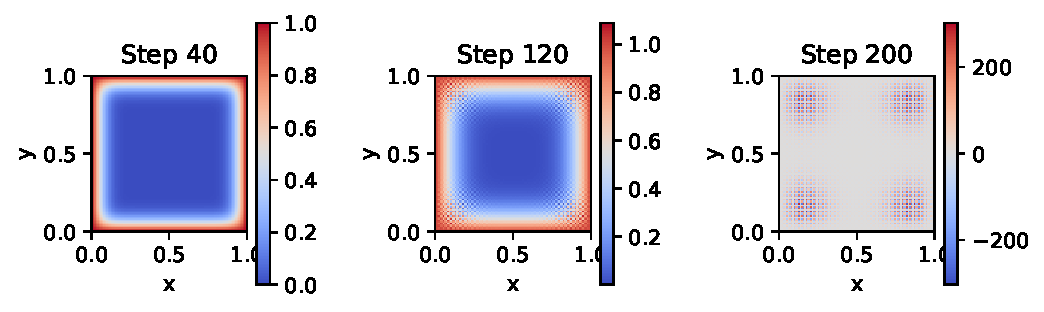
\includegraphics[width=\linewidth]{task_6_7_instability.pdf}
\caption{Instability at $r=0.2625$. Each panel has its own colour scale.
The early heat front looks reasonable; later panels show alternating grid-scale errors and growing extrema.}
\end{figure}
\textbf{Where it appears and what it looks like.}
In this experiment the visible oscillations first emerge in the boundary-heated regions near
the corners, before spreading farther into the plate. At step 120 a maximum occurs at grid
index $(i,j)=(4,59)$, near the upper-left corner. Symmetry produces equivalent regions near
the other corners, up to rounding. Alternating high and low values on neighbouring nodes form
a checkerboard. The location is specific to the initial and boundary data: if high-frequency
noise were inserted throughout the interior, the instability could appear there instead.

\begin{figure}[H]
\centering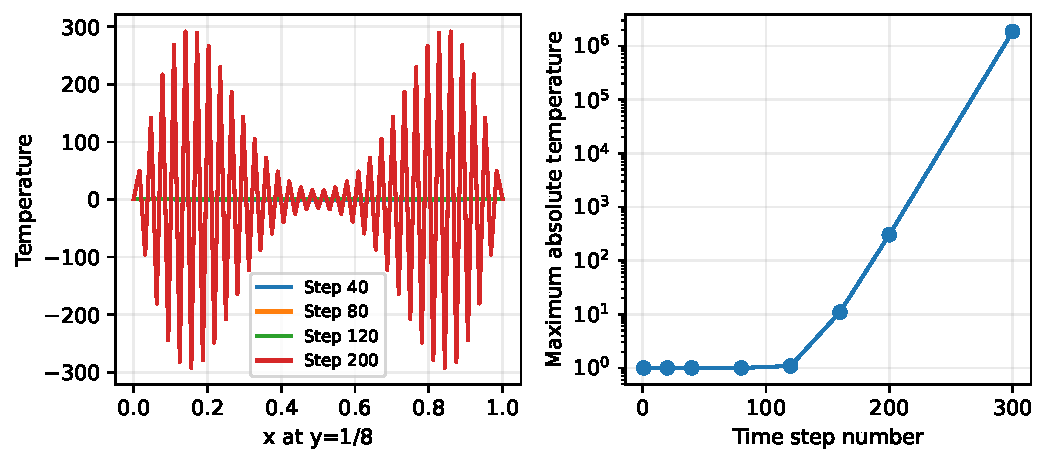
\includegraphics[width=\linewidth]{task_6_7_growth.pdf}
\caption{A horizontal cut at $y=1/8$ shows alternating values, while the maximum magnitude
eventually grows rapidly. Boundary values remain fixed at one throughout.}
\end{figure}
\textbf{Connection with the Fourier calculation.}
Task 6.3 gives the ideal checkerboard factor
\[
G(\pi,\pi)=1-8r=1-8(0.2625)=-1.1.
\]
Thus a checkerboard perturbation changes sign and grows by approximately $10\%$ each step.
After $n$ steps, its amplitude behaves like $(-1.1)^n$ in the Fourier model.
For the finite Dirichlet grid the highest sine mode instead has
\[
G_{\mathrm{highest}}=1-8r\cos^2\!\left(\frac{\pi}{2N}\right)
\simeq-1.09874\quad(N=64),
\]
which is still unstable. Its envelope and the superposition of nearby modes explain why the
actual field is not a uniform-amplitude checkerboard. Once this high-frequency component
dominates, the computation no longer represents heat diffusion.

\task{7.1}{Predicting the observed convergence order}
Task 5.5 gives first-order time error and second-order space error. For a stable method on a
smooth problem over a fixed time interval, the corresponding global estimate has the form
\[
E\le C_t\Delta t+C_xh^2+C_yh^2,
\]
with constants independent of the refined mesh sizes. Keeping
$r=\alpha\Delta t/h^2$ fixed means
\[
\Delta t=\frac{r}{\alpha}h^2.
\]
Substitute this relation into the error estimate:
\[
E\le\left(C_t\frac r\alpha+C_x+C_y\right)h^2.
\]
Therefore
\[
\boxed{E(h)=O(h^2),\qquad p_{\mathrm{predicted}}=2.}
\]
On halving $h$, the time step is quartered. Both time and spatial errors then decrease by
approximately four. Equivalently,
\[
\log_2\frac{E(h)}{E(h/2)}\longrightarrow2.
\]
This does not make forward Euler second order in time: its time error is still $O(\Delta t)$,
but the chosen refinement path makes $\Delta t$ proportional to $h^2$.
A special solution and parameter can cancel the leading error and produce an unusually high
observed order; the generic expectation remains two. Choosing $r=0.2$ in the next task avoids
the leading-error cancellation for the verification mode.

\task{7.2}{Convergence study}
\partsol{a}
We use the prescribed verification problem on $[0,1]^2$:
\[
u_0(x,y)=\sin(\pi x)\sin(\pi y),\qquad u=0\text{ on all four edges},\qquad\alpha=1,
\]
with exact solution
\[
u_{\mathrm{exact}}(x,y,t)=\sin(\pi x)\sin(\pi y)e^{-2\pi^2t}.
\]
The final time is $T=0.05$ and the fixed time-step parameter is $r=0.2<1/4$.
For each $N\in\{16,32,64,128,256\}$, set
\[
h=\frac1N,\qquad \Delta t=\frac{0.2}{N^2},\qquad
M=\frac{T}{\Delta t}=\frac{N^2}{4}.
\]
Every requested $N$ is even, so $M$ is an integer. Thus we keep $r$ exactly fixed and reach
the same $T$ exactly in the mathematical parameter specification, without rounding the step count.

\textbf{Implementation procedure.}
\begin{enumerate}
\item Allocate two contiguous double-precision arrays of $(N+1)^2$ values.
\item Initialize interior nodes from the sine product. Set all boundary entries to exactly zero
in both arrays; do not rely on floating-point evaluation of $\sin\pi$.
\item Apply the seven-operation update in Task 5.2(d) to every interior node for $M$ steps.
\item Swap the two array buffers after each step, keeping the old level intact during the update.
\item Evaluate the exact solution at the same nodes and final time, then compute both error norms.
\end{enumerate}
The reference program is C++17, compiled with optimization and floating-point contraction disabled.
It computes the full grid at every step; the table below is not generated solely from a modal formula.

\partsol{b}
Define the nodal error and the requested norms by
\[
e_{i,j}=u^M_{i,j}-u_{\mathrm{exact}}(x_i,y_j,T),
\]
\[
\norminf e=\max_{0\le i,j\le N}|e_{i,j}|,
\qquad
\normh e=\left(h^2\sum_{i=0}^N\sum_{j=0}^N e_{i,j}^2\right)^{1/2}.
\]
The factor $h^2$ makes the squared norm a quadrature approximation of a continuous integral.
Without it, changing the number of nodes would change the scale of the norm artificially.
Here the boundary errors are zero.

The observed order in a row compares that row with the preceding coarser grid, using
$\normh e$:
\[
p_{\mathrm{obs}}(N)=\log_2\frac{E(N/2)}{E(N)}.
\]
\begin{center}
\small
\begin{tabular}{rrrrrr}
\toprule
$N$ & $h$ & Steps & $\norminf e$ & $\normh e$ & $p_{\mathrm{obs}}$\\
\midrule
\tableinput{tables/task_7_2.tex}
\bottomrule
\end{tabular}
\end{center}
The time steps are, respectively,
\[
7.8125\times10^{-4},\quad1.953125\times10^{-4},\quad4.8828125\times10^{-5},
\]
\[
1.220703125\times10^{-5},\quad3.0517578125\times10^{-6}.
\]
\begin{figure}[H]
\centering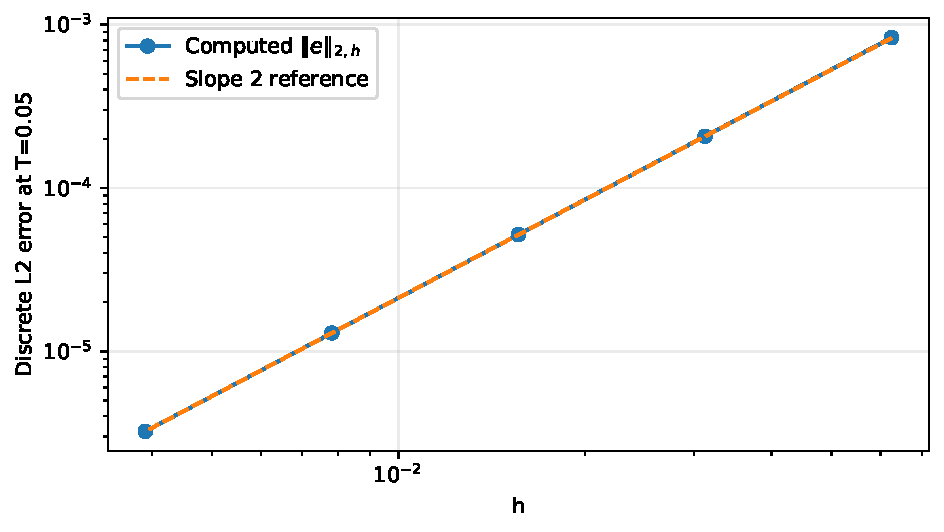
\includegraphics[width=.88\linewidth]{task_7_2_convergence.pdf}
\caption{Computed discrete $L^2$ error versus grid spacing at $T=0.05$, $r=0.2$.
The dashed line is proportional to $h^2$. Both axes are logarithmic.}
\end{figure}

\textbf{Independent analytical check of the computed table.}
For this initial condition, the sampled sine product is an eigenvector of the discrete Laplacian.
Its per-step factor is
\[
G_N=1-8r\sin^2\!\left(\frac{\pi}{2N}\right).
\]
Therefore, in exact arithmetic,
\[
u_{i,j}^M=G_N^M\sin\!\left(\frac{\pi i}{N}\right)
\sin\!\left(\frac{\pi j}{N}\right).
\]
Write $A_N=G_N^M-e^{-2\pi^2T}$. Then
$e_{i,j}=A_N\sin(\pi i/N)\sin(\pi j/N)$.
Because every $N$ in the table is even, the centre node has both sine factors equal to one:
\[
\norminf e=|A_N|.
\]
Also,
\[
\sum_{i=1}^{N-1}\sin^2\!\left(\frac{\pi i}{N}\right)=\frac N2.
\]
One way to see this is to use $\sin^2z=(1-\cos2z)/2$ and the vanishing sum of the $N$th
roots of unity. Applying this identity in both directions gives
\[
\normh e^2=h^2A_N^2\left(\frac N2\right)^2=\frac{A_N^2}{4},
\qquad
\boxed{\normh e=\frac12\norminf e.}
\]
The full-grid numerical results satisfy these modal predictions to within $5\times10^{-13}$
in absolute difference. This checks the stencil, step count, exact-solution evaluation, and
the normalization of the error norms independently of the observed slope.

\partsol{c}
The orders $2.00577$, $2.00144$, $2.00036$, and $2.00009$ approach two, as predicted in
Task 7.1. Both norms decrease by approximately a factor of four under each refinement.
The data therefore verify the expected convergence behaviour for this test.

The leading error can also be derived explicitly. For $h=1/N$,
\[
G_N=1-2r\pi^2h^2+\frac{r\pi^4}{6}h^4+O(h^6),
\]
so
\begin{align*}
\log G_N
&=-2r\pi^2h^2+\left(\frac r6-2r^2\right)\pi^4h^4+O(h^6),\\
M\log G_N
&=-2\pi^2T+\pi^4T\left(\frac16-2r\right)h^2+O(h^4),
\end{align*}
where $M=T/(rh^2)$. Consequently,
\[
A_N=e^{-2\pi^2T}\pi^4T\left(\frac16-2r\right)h^2+O(h^4).
\]
For $r=0.2$ this coefficient is nonzero and negative, so the leading error is truly second
order and the numerical mode decays a little faster than the exact one. For the special value
$r=1/12$, the leading error of this particular mode cancels; that is why a generic parameter
is preferable when using one exact mode to check the scheme's ordinary order.

\task{8.1}{Why an in-place update changes the method}
Assume rows are visited in increasing $j$, and columns within each row in increasing $i$.
Only the interior is updated; prescribed Dirichlet boundary values remain fixed.

\partsol{a}
When node $(i,j)$ is reached:
\begin{itemize}
\item The west neighbour $(i-1,j)$ has already been visited in the current row, so an interior
west neighbour contains level $n+1$ data.
\item The south neighbour $(i,j-1)$ belongs to an earlier row and also contains level $n+1$ data
when it is an interior unknown.
\item The east neighbour $(i+1,j)$ and north neighbour $(i,j+1)$ have not yet been visited,
so they still contain level $n$ data.
\item The centre still contains its old value until this update overwrites it.
\end{itemize}
At the first interior row or column, the corresponding south or west neighbour may instead
be a fixed boundary value. The issue concerns neighbours that are themselves updated unknowns.

\partsol{b}
Using one array would therefore apply the mixed-level relation
\[
u_{i,j}^{\mathrm{new}}=u_{i,j}^{\mathrm{old}}+r\left(
u_{i-1,j}^{\mathrm{new}}+u_{i+1,j}^{\mathrm{old}}
+u_{i,j-1}^{\mathrm{new}}+u_{i,j+1}^{\mathrm{old}}
-4u_{i,j}^{\mathrm{old}}\right).
\]
This is \emph{not} the forward-Euler scheme derived in Task 5.2, whose right-hand side must
use only level $n$. Reversing the traversal changes which neighbours are new, so the result
depends on the visitation order.

For a concrete example, consider the 1D three-interior-node row with zero endpoint values,
initial interior values $(1,0,0)$, and $r=0.1$:
\begin{center}
\begin{tabular}{lr}
\toprule
Update method & New interior values\\
\midrule
Correct simultaneous explicit update & $(0.8,\ 0.1,\ 0)$\\
In place, left to right & $(0.8,\ 0.08,\ 0.008)$\\
In place, right to left & $(0.81,\ 0.1,\ 0)$\\
\bottomrule
\end{tabular}
\end{center}
For example, in the left-to-right pass the second node reads the already changed first node,
so it receives $0.1\times0.8=0.08$ instead of $0.1\times1=0.1$.
The three different results demonstrate both the change in method and the order dependence.

\partsol{c}
When the domain is divided among processes, each process updates its own nodes, and their
relative execution order is not fixed. A valid explicit step must produce the same mathematical
result regardless of which process runs first. If updates read a mixture of old and new values,
the output depends on process boundaries, scheduling, and communication timing.

Use two arrays: read all stencil values from \texttt{old}, write all updated nodes into
\texttt{next}, then swap their buffers after the step. The swap exchanges array storage references;
it does not copy the full field. With consistent arithmetic order and correctly refreshed halos,
this preserves the serial update independently of how the grid is partitioned.

\task{8.2}{Surface-to-volume communication analysis}
For this scaling exercise, $N\times N$ denotes the grid size in the approximate counting sense
used by the question. The actual solver with $N$ intervals has $(N-1)^2$ interior unknowns;
replacing $N$ by the relevant exact row length changes lower-order terms, not the scaling.
We first consider a \emph{typical interior process}, meaning one with neighbours on both sides
of each decomposed direction. Physical-boundary processes have fewer messages.

Let
\[
t_{\mathrm{msg}}(m)=t_s+m t_w,
\]
where $m$ is a number of scalar values, $t_s$ is the message startup time, and $t_w$ is time
per scalar value. These are the units used in the background notes. If a network fit uses
bytes instead, then for doubles $t_w^{\mathrm{value}}=8t_w^{\mathrm{byte}}$.

\partsol{a}
\textbf{Strips.} Each process owns approximately $N/P$ complete rows, each of length $N$.
It needs one halo row above and one below. Therefore a typical interior process
\begin{itemize}
\item sends $N$ values to each of two neighbours: $2N$ values in total;
\item receives $N$ values from each of two neighbours: $2N$ received values;
\item issues two outgoing messages and receives two incoming messages per step.
\end{itemize}
Thus there are \textbf{four directed message events} locally, or \textbf{two bidirectional
neighbour exchanges}. Counting sent plus received values gives $4N$ scalar transfers per process.
An end strip has only one neighbour, and for $P=1$ there is no interprocess exchange.

\partsol{b}
\textbf{Square blocks.} Assume $P$ is a perfect square and processes form a
$\sqrt P\times\sqrt P$ grid. Each owns approximately
$(N/\sqrt P)\times(N/\sqrt P)$ nodes.
There is one halo edge in each of four directions, of length $N/\sqrt P$.
A typical interior process therefore
\begin{itemize}
\item sends $4N/\sqrt P$ values and receives $4N/\sqrt P$ values;
\item sends four messages and receives four messages per step.
\end{itemize}
This is eight directed message events, or four bidirectional neighbour exchanges.
The four corner ghost values are unnecessary for a five-point stencil, since no update reads
diagonal neighbours. A nine-point stencil with diagonal inputs would require additional data.

\partsol{c}
To turn these counts into time, the communication convention must be stated.
Assume each neighbour exchange has cost $t_s+m t_w$, send and receive can progress together
within that exchange, and the neighbour exchanges are completed in succession.
With this common full-duplex model,
\[
\boxed{T_{\mathrm{comm,strips}}\simeq2(t_s+Nt_w),}
\]
\[
\boxed{T_{\mathrm{comm,blocks}}\simeq4\left(t_s+\frac{N}{\sqrt P}t_w\right).}
\]
If instead the model charges separately for \emph{every directed send and receive with no
overlap}, both expressions double: $4(t_s+Nt_w)$ and
$8(t_s+(N/\sqrt P)t_w)$. Both conventions describe the same counts; their constants differ
because they assume different concurrency. One must use the convention consistent with how
the communication timing was measured.

\textbf{Small startup time.}
When bandwidth dominates, the ratio of these interior-process block and strip costs is
\[
\frac{4Nt_w/\sqrt P}{2Nt_w}=\frac{2}{\sqrt P}.
\]
For $P>4$, blocks communicate fewer values and are favoured by this model. Their area is the
same as a strip's, but their perimeter is smaller. For fixed $P=4$ the nominal interior-process
bandwidth terms coincide; actual boundary-neighbour counts must then be considered.

\textbf{Large startup time.}
If startup dominates both bandwidth terms, strips cost approximately $2t_s$, while an
interior block costs approximately $4t_s$. Strips can therefore be faster despite moving
more data. For the displayed interior-process formulas, blocks win exactly when
\begin{align*}
4t_s+\frac{4N}{\sqrt P}t_w&<2t_s+2Nt_w,\\
t_s&<Nt_w\left(1-\frac{2}{\sqrt P}\right).
\end{align*}
The right-hand side is positive only for $P>4$; this threshold belongs specifically to the
four-neighbour interior-block comparison, not to every finite process grid.

\textbf{Boundary-aware refinement.}
For a nonperiodic process grid, let $d_x$ be the number of left/right neighbours of a rank
and $d_y$ its number of lower/upper neighbours. On a $P_x\times P_y$ layout,
\[
T_{\mathrm{comm,rank}}\simeq
d_x\left(t_s+\frac{N}{P_y}t_w\right)
+d_y\left(t_s+\frac{N}{P_x}t_w\right).
\]
Each $d$ is zero, one, or two as appropriate. For example, on a $2\times2$ grid every rank
is a corner rank: it has two neighbours, not four. Its model cost is
$2t_s+Nt_w$. Four strips have middle ranks with cost $2t_s+2Nt_w$.
Thus the finite-grid block layout can have the same startup cost and less data even though
the generic four-neighbour formulas do not show this. This qualification prevents using an
interior-process approximation where no such interior process exists.

\partsol{d}
Let $c$ be the compute time per updated node per step. Balanced strips own approximately
$N^2/P$ nodes, so
\[
T_{\mathrm{comp}}\simeq c\frac{N^2}{P}.
\]
Using the paired-exchange convention above,
\begin{align*}
\frac{T_{\mathrm{comm,strips}}}{T_{\mathrm{comp}}}
&\simeq\frac{2(t_s+Nt_w)}{cN^2/P}\\
&=\boxed{\frac{2Pt_s}{cN^2}+\frac{2Pt_w}{cN}.}
\end{align*}
For fixed $P$, the latency contribution decreases as $N^{-2}$ and the bandwidth contribution
as $N^{-1}$. Larger grids therefore provide more computation per exchanged value, and the
communication fraction tends to decrease. At fixed $N$, increasing $P$ increases this ratio:
each rank computes less while it must still exchange full-length rows.

To make communication small compared with computation, one needs approximately
\[
N\gg\sqrt{\frac{2Pt_s}{c}},\qquad
N\gg\frac{2Pt_w}{c}.
\]
These conditions explain why small problems rarely benefit from a slow network, whereas a
sufficiently large grid may amortize the same startup costs. They are scaling criteria,
not measured crossover sizes. A simple idealized per-step strip model is
\[
T_P\simeq\frac{cN^2}{P}+2(t_s+Nt_w).
\]
Comparing with $T_1\simeq cN^2$ shows that a predicted speedup requires
\[
2(t_s+Nt_w)<cN^2\left(1-\frac1P\right).
\]
Actual crossover sizes also depend on load balance, memory behaviour, network contention,
and whether neighbour exchanges overlap. The area-to-perimeter argument explains the main trend.

\clearpage
\section*{Reproducibility and sources}
\textbf{Supplied computational files.}
The folder \texttt{experiments/} contains the serial C++17 heat solver
\texttt{heat\_serial.cpp} and the Python script \texttt{run\_experiments.py}.
The script generates the numerical tables and figures for Tasks 3.2, 3.5, 4.1, 6.7, and 7.2.
The directory \texttt{results/} contains CSV tables, raw heat-solver output, and binary snapshot fields.
The directories \texttt{tables/} and \texttt{figures/} contain the files included by this document.

On a system with a C++17 compiler, Python, NumPy, and Matplotlib, run from the document folder:
\begin{lstlisting}
g++ -std=c++17 -O3 -ffp-contract=off experiments/heat_serial.cpp -o experiments/heat_serial
python experiments/run_experiments.py
pdflatex -interaction=nonstopmode -halt-on-error Methode_Numerique_Tasks_Solutions.tex
\end{lstlisting}
On Windows, use \texttt{experiments/heat\_serial.exe} as the executable output name; the Python
script selects the corresponding executable automatically. For a compiler with a different
output location, pass its path as the script's first argument.

All reported numerical experiments use double precision. Timings recorded in the raw output
are incidental and are not used as project cluster-performance results. The seven-operation
counts in Task 6.6 are theoretical estimates under the stated sustained-rate assumption.
The instability experiment is deliberately isolated from the ordinary stability checks.

\textbf{Primary sources.}
\begin{enumerate}
\item \emph{Numerical Methods for the Heat Equation}, supplied course background notes,
Chapters 1--8. Task numbers, notation, input data, and requested experiments follow this document.
\item \emph{Parallel 2D Heat Diffusion with MPI over Tailscale}, supplied project specification,
Section 3 and Part 1. The boundary-heated initial data used in Task 6.7 and the serial-reference
implementation conventions follow this specification.
\end{enumerate}

\textbf{Assistance acknowledgement.}
OpenAI Codex assisted with the mathematical exposition, experimental C++/Python programs,
and LaTeX preparation.

\end{document}
